\section{Der Algorithmus von van Kreveld}

Die Laufzeit des naiven Algorithmus in $O(n^3)$ liegt (wobei $n$ das Maximum aus Breite und Höhe des DEM ist), gibt es einige Überlegungen zu 
schnelleren Algorithmen. Als eine Art untere Schranke für die Laufzeit der viewshed-Berechnung kann das Einlesen des DEMs gesehen werden, welches 
in $O(n^2)$ liegt. Somit sollte eine Verbesserung der Laufzeit möglichst nahe an diese untere Schranke heranreichen. Im Paper von van Kreveld 
\cite{vanKrev} werden Optimierungsvorschläge vorgestellt und gezeigt, dass die Laufzeit auf $O(n^2)\log n$ verbessert werden kann. 

\subsection{Der sweep line-Algorithmus}
Van Krevelds Algorithmus beruht auf dem Prinzip der sogenannten ``sweep line''. Allgemein ist eine sweep line eine (horizontale) Linie, 
welche über eine Menge von Objekten in einer Ebene ``streicht'' und dabei alle relevanten Informationen bezüglich einer Problemstellung ausliest und 
sammelt, damit diese dann weiterverarbeitet werden können. Beispielsweise kann die Linie über eine Ebene streichen und dabei den Beginn und das Ende 
geometrischer Formen detektieren (siehe Abbildung \ref{sweep}). Da sich die Menge der Objekte, die die Linie schneiden, oft ändert, muss für das 
Sammeln der Informationen eine flexible Datenstruktur gewählt werden. Hierfür eignet sich ein balancierter binärer Baum, welcher als 
``Statusstruktur'' bezeichnet wird (siehe Abbildung \ref{stat}) und die Änderungen des Status festzuhalten. 

\begin{figure}[!ht]
\begin{minipage}{0.55\textwidth}
\centering
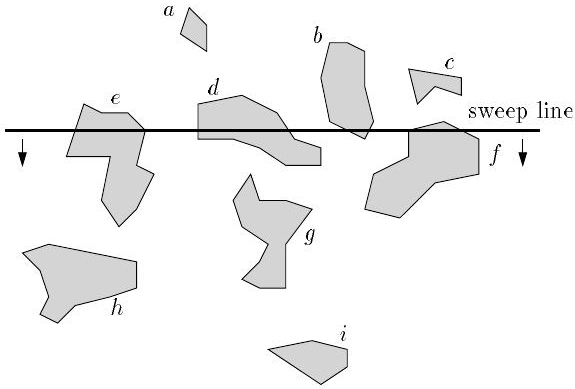
\includegraphics[scale=0.62]{bilder/sweep}
\caption{sweep line streicht über Objekte in einer Ebene}
\label{sweep}
\end{minipage}
\hfill
\begin{minipage}{0.4\textwidth}
\centering
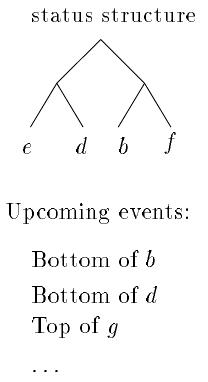
\includegraphics[scale=0.67]{bilder/statstruc}
\caption{Statusstruktur, in der die auftretenden Ereignisse gespeichert werden}
\label{stat}
\end{minipage}
\end{figure}

Um zu wissen, wann sich der Status ändert -- also wenn die Linie beispielsweise ein neues Objekt schneidet -- werden sogenannte ``events'' eingeführt
und ebenfalls in einer eigenen Datenstruktur gespeichert. Hierfür kann eine Prioritätswarteschlange oder ebenfalls ein balancierter binärer Baum 
benutzt werden. Für das Beispiel der viewshed-Analyse ist die Definition folgender events sinnvoll: 
\begin{itemize}
 \item die sweep line detektiert beim Streichen über das DEM einen neuen Pixel
 \item die sweep line detektiert beim Streichen über das DEM den Mittelpunkt eines Pixels
 \item die sweep line detektiert beim Streichen über das DEM die ``letzte Ecke'' eines Pixels, er wurde also von der Linie komplett durchlaufen
\end{itemize}

Der Pseudocode für den sweep line-Algorithmus ist in Abbildung \ref{pseudo} zu sehen.
\vspace{5pt}

Aufgrund der gewählten Datenstruktur eines balancierten binären Baums für die Statusstruktur erfolgt das Einfügen und Löschen von Daten sowie der 
Zugriff darauf in $O(\log n)$ Zeit, wodurch hier gegenüber dem naiven Algorithmus eine deutliche Verbesserung der Laufzeit erreicht wird. Das 
Einlesen des DEMs erfolgt weiterhin in $O(n^2)$ Zeit, doch durch das Benutzen des sweep line-Algorithmus kommt nun nur noch ein Anteil von 
$O(\log n)$ hinzu, was in einer Gesamtlaufzeit von $O(n^2\log n)$ resultiert.

\begin{figure}[!ht]
 \centering
 \begin{BVerbatim}
Initialisiere die event list und die Statusstruktur
 Solange die event list noch nicht leer ist 
  Do Nimm das erste Element aus der Liste 
     Wenn ein neues Objekt die sweep line schneidet
	       füge es in die Statusstruktur ein
     Wenn ein Objekt nicht länger von der sweep line geschnitten wird
	       lösche es aus der Statusstruktur heraus
     Falls möglich, führe die gewünschten Berechnungen mit Hilfe der Statusstruktur durch      
     Falls nötig, füge neue events in die event list ein
  EndDo
\end{BVerbatim}
\caption{Pseudocode für sweep line-Algorithmus}
\label{pseudo}
\end{figure}

\subsection{Anpassung des sweep line-Algorithmus für das Problem der viewshed-Analyse}
\label{sweep_adjust}
Um den sweep line-Algorithmus für die viewshed-Analyse benutzen zu können, müssen ein paar kleine Anpassungen vorgenommen werden. Im Gegensatz zu 
der in Abbildung \ref{sweep} gezeigten horizontalen sweep line, legt van Kreveld den Ursprung der Linie auf die Koordinaten des Standorts und lässt 
sie dann wie bei einem Radar in einer Kreisbewegung über das DEM streichen (siehe Abbildung \ref{sweep_k}).

\begin{figure}[!ht]
 \centering
 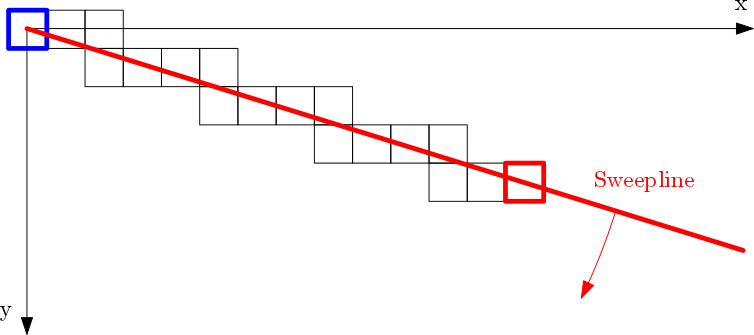
\includegraphics[scale=0.45]{bilder/sweep_kreveld}
 \caption{Definition der sweep line im Algorithmus von van Kreveld. Der Standort ist blau markiert, der rot umrandete Pixel ist ein Randpixel des 
 DEMs.}
 \label{sweep_k}
\end{figure}

In unserer Implementierung definieren wir den Winkel $0^\circ$ für die sweep line parallel zur x-Achse und sie schneidet zu Beginn des Algorithmus 
alle Pixel rechts neben dem Standort. Zudem lassen wir die Linie -- wie die Abbildung zeigt -- \textbf{im} Uhrzeigersinn über das DEM kreisen. Im 
Gegensatz zur ``normalen'' sweep line, ist hier die Länge der sweep line nicht konstant, sondern hängt vom Setzen des Standorts im DEM ab. 

Weiterhin haben wir drei Klassen von events definiert: 
\begin{itemize}
 \item \textit{EventType\_IN}: die sweep line detektiert den Beginn eines Pixels im DEM 
 \item \textit{EventType\_CENTER}: die sweep line streicht über die Mitte eines Pixels,
 \item \textit{EventType\_OUT}: die sweep line detektiert das Ende eines Pixels im DEM, also die letzte Ecke, die überstrichen wird
\end{itemize}

Für jeden Pixel im DEM wird der Winkel zum Standort berechnet, unter dem die drei jeweiligen Eventtypen auftreten. Dies ist nötig, da alle Eventtypen 
in der event list nach dem Winkel zum Standort sortiert werden. Somit wird das Prinzip der kreisförmigen Bewegung der sweep line realisiert, da die 
Pixel der Reihe nach mit aufsteigendem Winkel abgearbeitet werden. 

Die Berechnung, ob ein Pixel vom Standort aus sichtbar ist, erfolgt mit Hilfe der Statusstruktur, welche in Kapitel \ref{tree} genauer beschrieben 
ist.

Unsere (erste) Implementierung des van Kreveld-Algorithmus lässt sich folgendermaßen als Pseusocode darstellen:

\begin{figure}[!ht]
 \centering
 \begin{BVerbatim}
  Initialisiere die Statusstruktur 
  Fülle die event list, indem für jeden Pixel im DEM die drei entsprechenden Eventtypen 
    in die event list eingefügt werden  
  Solange die event list noch nicht leer ist 
    Do Nimm das erste event aus der Liste 
      Falls Typ == EventType.IN
	  füge Pixel in die Statusstruktur ein
      Falls Typ == EventType.OUT
	  lösche Pixel in der Statusstruktur 
      Falls Typ == EventType.CENTER
	  berechne die Sichtbarkeit des Pixels mit Hilfe der in der Statusstruktur 
	  gespeicherten Daten
    EndDo

 \end{BVerbatim}
 \caption{Pseudocode für van Kreveld-Algorithmus}
 \label{pseudo_krev}
\end{figure}

Nach der Implementierung dieses Codes zeigten bereits die ersten Testläufe, dass dieser Algorithmus trotz der angepriesenen Verbesserung der Laufzeit 
wesentlich länger zur Berechnung eines viewsheds benötigte, als der naive Algorithmus. Im folgenden Kapitel werden unter Punkt \ref{speicher} daher 
die von uns identifizierten Probleme des Codes dargestellt und Lösungsvorschläge unterbreitet. 

